\documentclass[10pt,twocolumn,letterpaper]{article}

\usepackage{cvpr}
\usepackage{times}
\usepackage{epsfig}
\usepackage{graphicx}
\usepackage{amsmath}
\usepackage{amssymb}
\usepackage{listings}
\usepackage{float}
\usepackage{subfigure}
% Include other packages here, before hyperref.

% If you comment hyperref and then uncomment it, you should delete
% egpaper.aux before re-running latex.  (Or just hit 'q' on the first latex
% run, let it finish, and you should be clear).
\usepackage[colorlinks,linkcolor=blue,urlcolor=blue,breaklinks=true,bookmarks=false]{hyperref}

\cvprfinalcopy % *** Uncomment this line for the final submission

\def\cvprPaperID{****} % *** Enter the CVPR Paper ID here
\def\httilde{\mbox{\tt\raisebox{-.5ex}{\symbol{126}}}}

% Pages are numbered in submission mode, and unnumbered in camera-ready
%\ifcvprfinal\pagestyle{empty}\fi
\setcounter{page}{1}

\lstset{
    language = python,
    columns = flexible,
    basicstyle = \tt\small,
    keywordstyle = \color{blue}\bfseries,
    identifierstyle = \color{black},
    commentstyle = \color[RGB]{80,80,80},
    numberstyle = \color{yellow}
}
\begin{document}

%%%%%%%%% TITLE
\title{CS182: Introduction to Machine Learning: \\ Image Super Resolution}

\author{Bi Chunhao, Jiang Yichen\\
% xxxxxxxxxx\\
%Institution1\\
Shanghaitech University\\
%Institution1 address\\
 {\tt\small \{bichh, jiangych\}@shanghaitech.edu.cn}
% For a paper whose authors are all at the same institution,
% omit the following lines up until the closing ``}''.
% Additional authors and addresses can be added with ``\and'',
% just like the second author.
% To save space, use either the email address or home page, not both
%\and
%Second Author\\
%Institution2\\
%First line of institution2 address\\
%{\tt\small secondauthor@i2.org}
}

\maketitle
%\thispagestyle{empty}

%%%%%%%%% ABSTRACT
\begin{abstract}
This is the final project of CS182, here we focused on a specific application called Image Super Resolution,
which generates a higher resolution images based on the raw input. 
We compared several existing algorithms and carried out some experiments to find the most suitable solution.
\end{abstract}

%%%%%%%%% BODY TEXT
\section{Introduction}

\section{Related Work}
\subsection{CNN methods}
\subsection{GAN}

\section{Networks} 
\subsection{Bicubic}

\subsection{FSRCNN}
FSRCNN[1] is also called fast-SRCNN. 
It is designed by Chao Dong, Chen Change Loy, and Xiaoou Tang, 
who first put forward applying deep learning neural network to super-resolution. 
\begin{figure}[H]
    \centering
    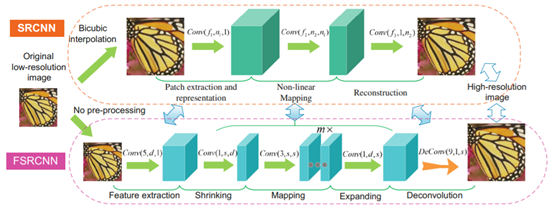
\includegraphics[scale = 0.4]{images/FSRCNN.png}
    \caption{The network structure of SRCNN and FSRCNN}
\end{figure}
Fast-SRCNN accelerating the current SRCNN[6]. SRCNN upscales LR image to target size by bicubic interpolation before actually entering the network. While FSRCNN just take LR image as the input, and conducts upsampling by the deconvolution layer at the end of the net work. This change leads to 2 main difference: 1. Directly, no need to cost time carrying out Bicubic operation. 2. Conv operation on LR image is less costly, With less computational complexity, FSRCNN can support a deeper network and achieve a better effect.
FSRCNN takes LR images as the input and carry out feature extraction. Then, replacing the non-linear mapping step, FSRCNN takes shrinking, mapping and expanding steps instead. And finally construct the desired HR image with a deconvolution operation. 
FSRCNN take PReLU as the activation function and L2 as loss.

\subsection{ESPCN}
ESPCN[2] is also motivated by SRCNN[6], like FSRCNN[1], ESPCN takes LR images as the input and have low computational complexity. 
\begin{figure}[H]
    \centering
    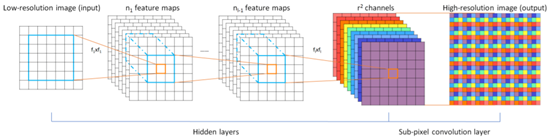
\includegraphics[scale = 0.4]{images/ESPCN.png}
    \caption{The network structure of ESPCN}
\end{figure}
The author team implement a more efficient sub-pixel convolution layer for learn. ESPCN takes an LR image as the input. For a network with L layers, ESPCN will learn L-1 upscaling filters for every channel, and finally a deconvolution layer that recovering resolution of the image. The use of deconvolution layer had shown good effect in other in visual field and cause low cost, that’s why both FSRCNN and ESPCN choose to use deconvolution layer. And operation also enable cheaper convolution operation to be use in hidden layers.
ESPCN take $tanh()$ as activation function and L2 as loss.

\subsection{LapSRN}
LapSRN's full name is Laplacian Pyramid Super-Resolution Network[3]. 
In comparison previous 2 model, LapSRN have deeper network structure, and has many properties. 
\begin{figure}[H]
    \centering
    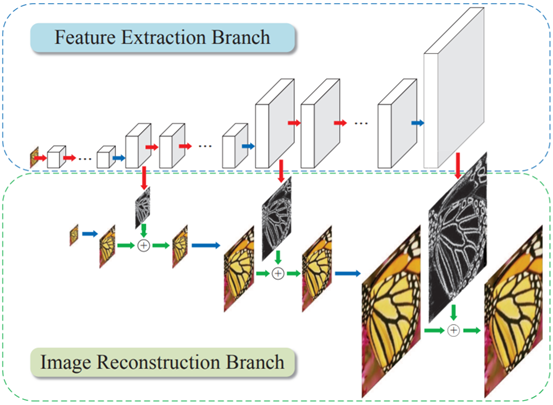
\includegraphics[scale = 0.4]{images/LapSRN.png}
    \caption{The network structure of LapSRN}
\end{figure} 

Despite the detailed network implementation, LapSRN have 3 main characteristic.
	1. LapSRN has multiple-level structure, every structure can conduct a 2x upscaling on input image and output of previous level can be taken as input of next level. As a result, LapSRN can support up to 8x upscaling, while most model only support 4x. 
2. In each level, feature extraction conduct first, then upscaling by a deconvolution layer to 2x size. LapSRN also motivated by Residual Learning[7], the upsampled image is then combined (using element-wise summation) with the predicted residual image from the feature extraction branch to produce a high-resolution output image.[3]
3. The author team think L2 loss is not good enough for SR learning and s inevitably
generate blurry predictions. So, LapSRN choose another loss: Charbonnier penalty function (a differentiable variant of L1 norm)[3]. This loss is considered at the end of every level.


\subsection{EDSR}
The design of EDSR is based on the SRResNet[8], which is motivated by ResNet[7] and achieve good performance in solving time/memory issue in SR.[4] What's more EDSR has won NTIRE2017 SR Challenge.
\begin{figure}[H]
    \centering
    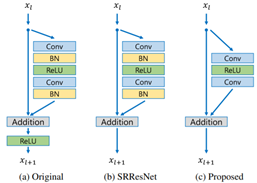
\includegraphics[scale = 0.6]{images/EDSR1.png}
    \caption{Comparison of residual blocks in ResNet, SRResNet and EDSR}
\end{figure} 
\begin{figure}[H]
    \centering
    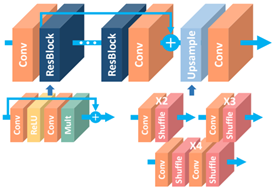
\includegraphics[scale = 0.6]{images/EDSR2.png}
    \caption{The architecture of the proposed single-scale SR network (EDSR)}
\end{figure} 
the author team find the batch normalization layers get rid of range flexibility from networks by normalizing the features. Since SR is low-level computer visual problem. These BN block in original ResNet may not do good for SR. So, EDSR remove these BN layers is better, which further lead to approximately 40% of memory usage saving.[4]
	EDSR use L1 loss instead of L2, because author team find L1 loss provides better convergence.



\section{Results and Experiments}
\subsection{Testing}
\subsubsection*{Models}
Due to time and equipments limitations, we can't train all the models by ourselves, so
we take the $\times 4$ version trained models of 
\href{https://github.com/Saafke/EDSR_Tensorflow/tree/master/models}{EDSR},
\href{https://github.com/Saafke/FSRCNN_Tensorflow/tree/master/models}{FSRCNN},
\href{https://github.com/fannymonori/TF-ESPCN/tree/master/export}{ESPCN},
\href{https://github.com/fannymonori/TF-LapSRN/tree/master/export}{LapSRN} from GitLab.

\subsubsection*{Evaluation Metrics}
\begin{itemize}
    \item PSNR 
    
    PSNR (Peak Signal to Noise Ratio) is a generally used measuring method for image resolution.
    PSNR is the ratio of maximum signal power and the average power.
    The definition is:
    \begin{align*}
        PSNR = 10log_{10}\frac{MaxValue^2}{MSE} = 10log_{10}\frac{255}{MSE}
    \end{align*}
    Where MSE(Mean Squared Error) denotes the average power between the groundtruth and the result image.

    However, PSNR scores is not consistent to the quality human eye perceives, sometimes a higher PSNR score image may look worse.
    The reason is that human eye is not sensitive to high frequency noise, which is usually separately distributed. 
    The perception is influenced by the whole surrounding area in a low frequency way.
    Below is some images with same PSNR scores, but is quite different for human perception. 
    \begin{figure}[H]
        \centering
        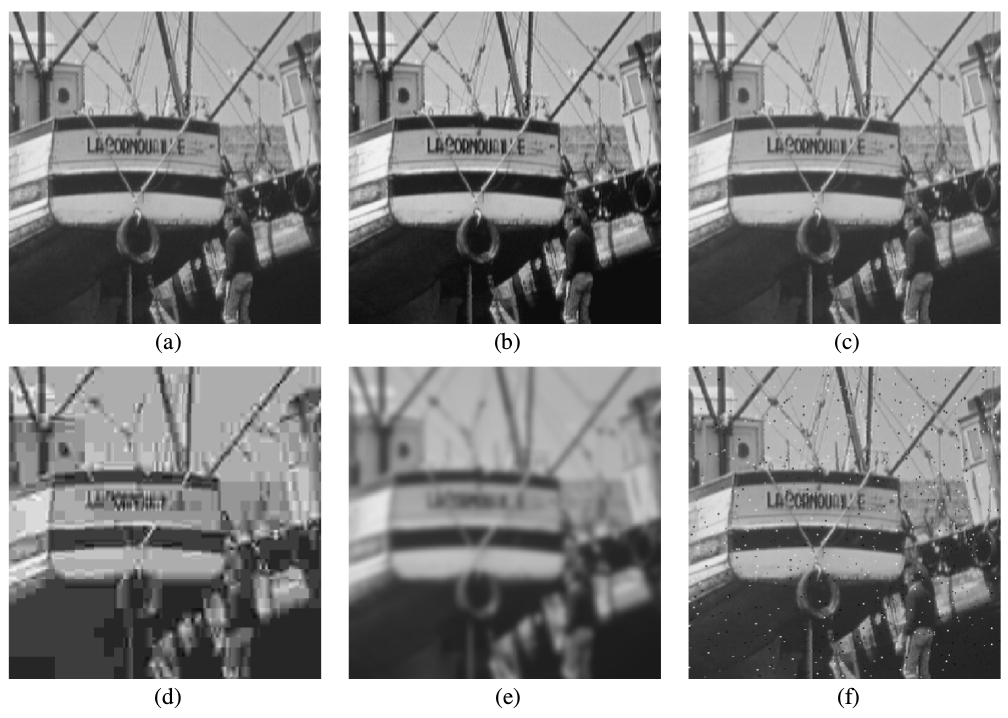
\includegraphics[scale = 0.3]{images/PSNR.png}
        \caption{Same PSNR scores with different distortions}
    \end{figure}

    \item SSIM
    
    SSIM (Structural Similarity Index) is a method to evaluate the similarity of two images.
    It is based on the whole structure, with less focus on pixelwise error. 
    SSIM contains three evaluation aspects:
    \begin{itemize}
        \item Luminance
        \item Contrast
        \item Structure
    \end{itemize}
    The detailed calculation is complicated. A general pipeline is as follows:
    \begin{figure}[H]
        \centering
        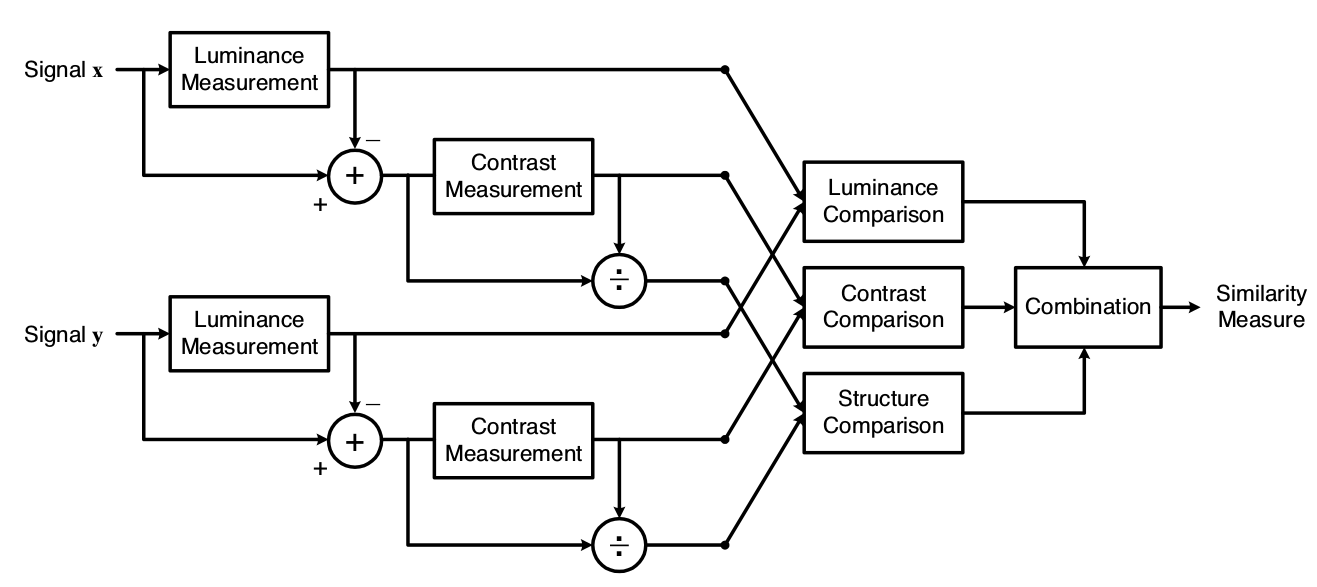
\includegraphics[scale = 0.2]{images/SSIM.png}
        \caption{Same PSNR scores with different distortions}
    \end{figure}
    The Luminance can be represented as mean value, the Contrast as variance after normalization, 
    and the structure as coefficient of association (fraction of covariance and variance products).

\end{itemize}


\subsection{Results}
The testing set we take is DIV2K High Resolution dataset \href{https://data.vision.ee.ethz.ch/cvl/DIV2K}{DIV2K\_valid\_HR}, 
which contains 100 2K images.
We first downsample the images to 1/4 size, and then use the model to generate images with origin resolution.
The evaluation result is calculated with the groundtruth image.
The average scores are as follows:
\begin{table}[H]
    \centering
    \caption{Image Evaluation on different networks}
    \begin{tabular}{|l|l|l|l|}
    \hline
    Average Evaluation  & PSNR   & SSIM   & Time spent  \\ \hline
    Bicubic             & 26.228 & 0.7722 & 0.0025      \\ \hline
    EDSR                & 27.789 & 0.8091 & 34.844      \\ \hline
    ESPCN               & 26.689 & 0.7737 & 0.0840      \\ \hline
    FSRCNN              & 26.580 & 0.7704 & 0.1302      \\ \hline
    LapSRN              & 26.710 & 0.7741 & 2.9266      \\ \hline
    \end{tabular}
\end{table}
To be noticed, EDSR results in a great accuracy. 
However, due to the great size of its network, it also spent a lot of time than the others.


\subsection{Visualization}
If the scores are not familiar, some visual results can bring a more intuitive understanding.
\begin{figure}[H]
    \centering
    \subfigure[Origin]{
    \begin{minipage}[t]{0.3\linewidth}
    \centering
    
\includegraphics[width=1in]{images/plant_origin.png}
    \end{minipage}
    }
    \subfigure[Bicubic]{
    \begin{minipage}[t]{0.3\linewidth}
    \centering
    
\includegraphics[width=1in]{images/plant_bicubic.png}
    \end{minipage}
    }
    \subfigure[EDSR]{
    \begin{minipage}[t]{0.3\linewidth}
    \centering
    
\includegraphics[width=1in]{images/plant_EDSR.png}
    \end{minipage}
    }

    \subfigure[ESPCN]{
    \begin{minipage}[t]{0.3\linewidth}
    \centering
    
\includegraphics[width=1in]{images/plant_ESPCN.png}
    \end{minipage}
    }
    \subfigure[FSRCNN]{
    \begin{minipage}[t]{0.3\linewidth}
    \centering
    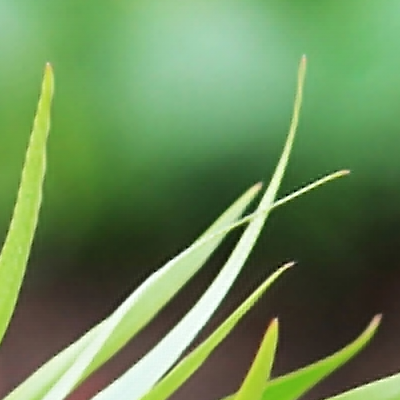
\includegraphics[width=1in]{images/plant_FSRCNN.png}
    \end{minipage}
    }
    \subfigure[LapSRN]{
    \begin{minipage}[t]{0.3\linewidth}
    \centering
    
\includegraphics[width=1in]{images/plant_LapSRN.png}
    \end{minipage}
    }
    \caption{Restoration from aliased compression}
\end{figure}
From the result above, we can tell that the model is useful for dealing with aliasing.
Aliasing is a normal consequence when pictures are compressed into a lower resolution.
The bicubic interpolation can't do well with this situation, 
but the rest four methods can smoothen the images to be more realistic.

\section{Conclusion}

{\small
\bibliographystyle{ieee_fullname}
\bibliography{reportbib}
}



\end{document}
